% Chapter Template

\chapter{Network Components and Protocols} % Main chapter title

\label{Chapter3} % Change X to a consecutive number; for referencing this chapter elsewhere, use \ref{ChapterX}

\lhead{Chapter 3. \emph{Network Components and Protocols}} % Change X to a consecutive number; this is for the header on each page - perhaps a shortened title

%----------------------------------------------------------------------------------------
%	SECTION 1
%----------------------------------------------------------------------------------------
The purpose of this chapter is to present the different protocols or concepts that are used throughout this thesis.

\section{EAP}
\texttt{EAP} (\textit{The Extensible Authentication Protocol}) is a flexible authentication framework defined on the RFC3748 \cite{rfc3748}. EAP was designed to work without the IP protocol and provides support only for the transport of authentication protocols. The idea behind EAP was to creates a framework that supports several authentication methods and to separates the ahtentication methods from the transport.

\section{IEEE 802.1X}
%http://www.blackhat.com/presentations/win-usa-03/bh-win-03-riley-wireless/bh-win-03-riley.pdf
\texttt{802.1X} is a Port-based Network Access Control that is part of the \texttt{IEEE 802.1} group of networking protocols. Basically, it is a way of securing a network access and doing authentication over ports to devices wishing to attach to a LAN or a WLAN. It offers an effective framework for authenticating and controlling user traffic to a protected network.

The \texttt{802.1X} authentication process architecture involves three main components:
\begin{itemize}
	\item[-]\texttt{A supplicant}: The client device that wants to connect to the network (LAN or WLAN).
	\item[-]\texttt{An authenticator}: A network device like an Ethernet switch or an access point that is between the supplicant and the authentication server. It purpose is to interact with the authentication server. It receives \texttt{EAP} messages, encapsulates them into \texttt{RADIUS} messages and forwards them to the authentication server.
	\item[-]\texttt{An authentication server}: It is the key part of that authentication process. This server support receives the authentication request from the authenticator and interacts with him in order to receive more information or credentials for the supplicant. It is the only one that can grant access or not to the protected network to the user.
\end{itemize} 

This protocol is called \textit{Port-based Network Access Control} because the ports of the switches are configured in a certain way. Indeed, before being totally open, they only accept \texttt{EAP} messages. The idea is that each port is divided into two different parts. One part is the \textit{controlled} part of the port and the other is the \textit{uncontrolled} part of the port. The main idea is that all the \texttt{EAP} messages go through this uncontrolled port.

\texttt{802.1X} works either for WLAN or LAN authentication but the authentication flow is not exactly the same.
For WLAN authentication, the first thing the supplicant does is to associate with the access point using standard \texttt{802.11} communication. It then sends its information inside \texttt{EAP} messages to the authenticator through the uncontrolled port. The authenticator encapsulates those messages into \texttt{RADIUS} packets and sends them to the authentication server. Then, after having set up a secure and encrypted tunnel with the supplicant, the authentication server starts communicating with it (to receive its username and password for example). The server then queries its database and finally, if the user is know, it asks the autenticator to open completely the port so that the user can access the requested VLAN.
The following figure represents this authentication mechanism for WLAN.

\begin{figure}[H]
	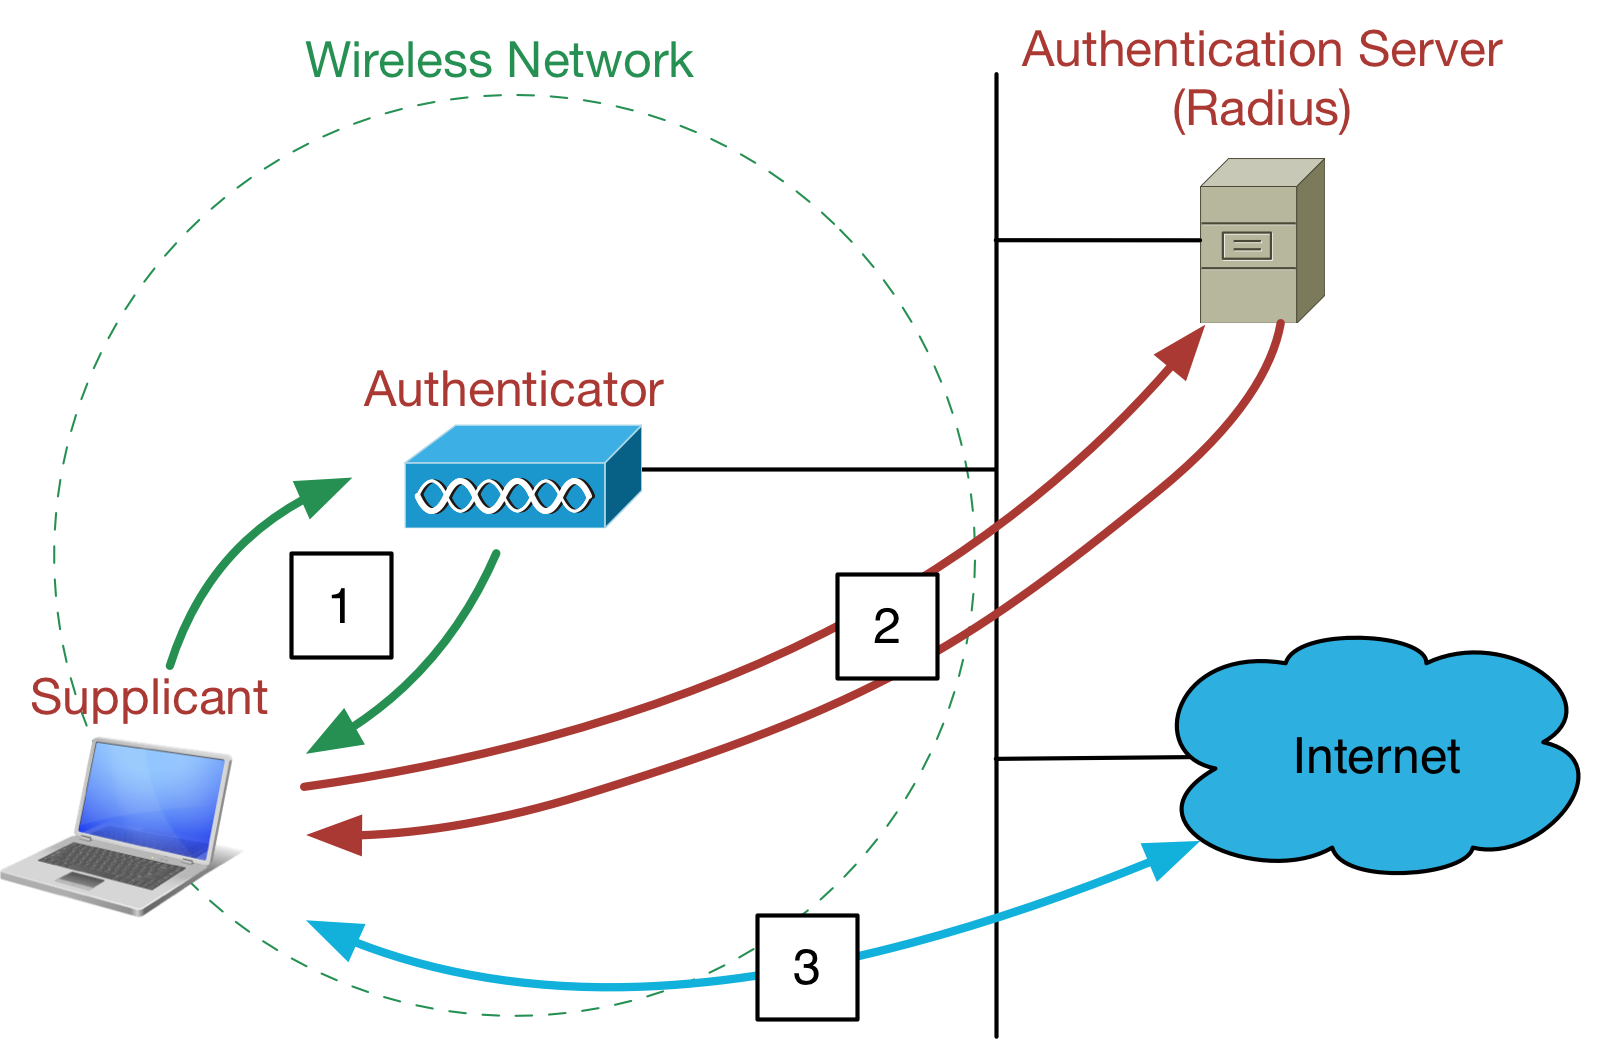
\includegraphics[width=.7\linewidth]{Pictures/Chapter3/802.png}
	\caption{\texttt{802.1X} authentication mechanism for WLAN}
\end{figure}

For LAN authentication it is a bit different. Indeed, the user directly connects to the switch through Ethernet. The switch then passes all the supplicant information to the authentication server. The authentication server and the switch exchange authentication and then the server queries its database and asks the switch to open the port or not.
We can see that there is a major difference between WLAN and LAN authentication mechanisms. Indeed, in LAN, there are absolutely no communications between the authentication server and the supplicant. All the communications are done only between the switch and the server, while in WLAN, the authentication server directly communicates with the supplicant through a secured and an encrypted tunnel. 



\section{RADIUS}


\section{WiSM}


\section{SNMP}

The Simple Network Management Protocol is an application layer protocol that facilitates the exchange of management information between network devices \cite{snmp}. It is part of the TCP/IP protocol suite and it is mainly used by network administrators to get information about devices on the network and the network performances. These information help the administrators to resolve problems on the network or simply to manage it.
A SNMP network has three main components:

\begin{itemize}
	\item \texttt{Network-management system (NMS)}: A NMS is the main component of an SNMP-managed network. It is the management entity that controls the managed devices. It uses the SNMP protocol and can interact with the managed devices to get information using special commands and messages.
	
	\item \texttt{Managed devices}: It is a network device that contains an SNMP agent. They collect and store information to make them available for the network-management systems. Those devices can be routers, servers, switches,etc. They also run the SNMP protocols to be able to respond to the requests made by the NMS.
	
	\item \texttt{Agents}: An agent is the thinking part of a managed device. It is a software module that understands the management information and translates them into a SNMP compatible form.
\end{itemize}

\begin{figure}[H]
\centering
	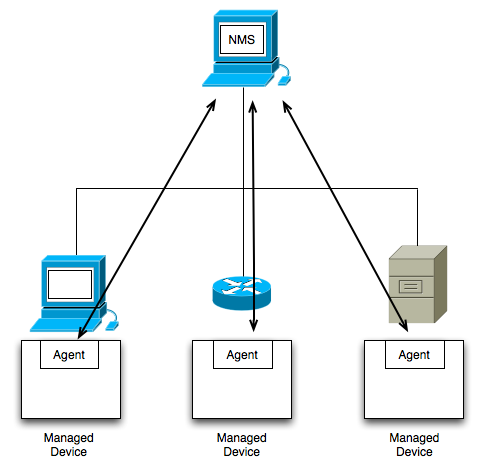
\includegraphics[width=.7\linewidth]{Pictures/Chapter3/snmp.png}
	\caption{A typical SNMP managed network}
\end{figure}

All the network objects are described and organized hierarchically in a Management Information Base (MIB). There are MIBs for each set of related network entites that can be managed. These MIBs are accessed using a network-management protocol such as SNMP.

